% !TeX spellcheck = fr_FR
\documentclass[final]{article}
\usepackage{multicol}
\usepackage[a4paper, total={5.8in, 9.5in}]{geometry}
\usepackage[french]{babel}
\usepackage[utf8]{inputenc}
\usepackage[T1]{fontenc}
\usepackage{graphicx}
\usepackage{mdframed}
\usepackage{etoolbox}
\usepackage{qrcode}
\usepackage{vwcol}
\usepackage{float}
\usepackage{qrcode}
\usepackage{amsmath}
\usepackage{listings}
\usepackage{tabularx}
\usepackage{pdfpages}
\usepackage{lastpage}

\newcommand{\code}[1]{
    \boxed{\texttt{#1}}
}

\title{G31---Stratégie de tests T3}
\author{KOCAK Mikail, GROSJEAN Martin, et Razafindratsita Loïc}
\date{19 octobre 2018}

%%% Custom headers and footers using the 'fancyhdr' package
\usepackage{fancyhdr}
\pagestyle{fancyplain}
\pagestyle{fancy}
\fancyhead{}
\fancyfoot[L]{\small{KOCAK Mikail\\GROSJEAN Martin\\Razafindratsita Loïc}}
\fancyfoot[C]{}
\fancyfoot[R]{Page \thepage ~sur \pageref{LastPage}}


\begin{document}

  \maketitle
  
  \tableofcontents
  
  \section{Courte introduction}
    Urbanotopus est un \emph{Visual Novel} où le joueur se fond dans l'histoire 
    d'un urbaniste avec une multitude de choix menant 
    à une infinité de dénouements de l'histoire.

    L'objectif de ce jeu est d'apprendre au joueur les implications de chaque choix 
    et donc l'important qu'à et que les choix, parfois difficiles de l'urbaniste ont.\\
    
    Chaque jour, le joueur est présenté à un nouveau scénario ou 
    un scénario qui continu le dernier joué. 
    Dans ces scénarios, le joueur doit prendre une ou des actions 
    qui modifient les variables de sa partie.
    Ces situations et décisions peuvent influencer en bien ou en mal
    la partie du joueur en fonction de ses décisions.

    Le joueur peut très facilement juger de ses performances à partir des conséquences, 
    mais aussi en lisant ce que les gens postent sur le flux Twitter. 
    Mais encore en regardant les chaînes d'informations, la radio et enfin, 
    en regardant les statistiques de la partie.
  
  \section{Exigences de tests sur le projet}
    \subsection{
        Contrôle qualité et tests avant fusion des proposition de codes}      
      \indent Tout d'abord, les changements du code 
      sont automatiquement testés et refusés ou acceptés par 
      des séries de tests entrepris par les logiciels de CI 
      (\emph{continuous integration}). Ils se définissent par :

      \begin{enumerate}
        \item \textbf{Le code se compile et s'installe} correctement sur 
        tous les systèmes ciblés (MacOS, Linux et Windows) ;
        \item Et \textbf{les \emph{tests unitaires} aboutissent avec succès}
        sur toutes ces machines ;
        \item \textbf{Le \emph{code coverage} ne baisse pas}.
      \end{enumerate}
      
      \indent Ensuite, le projet a des règles strictes pré-définies 
      sur comment contribuer au code source du projet. Qui a pour but
      d'assurer et d'expliquer comment assurer la qualité 
      et donc tester la qualité et maintenance du code.
        
      \indent L'objectif étant d'imposer un contrôle humain
      stricte à ce qu'on puisse assurer une qualité maximale
      et un risque de bug minimal.
        
      \begin{vwcol}[widths={0.85,0.15}, sep=.2cm, justify=flush,rule=0pt,indent=1em]
        \indent Aucune fusion du code n'est acceptée s'il n'a pas été
        testé et affirmé comme fonctionnel et 
        aucun problème ne semble se manifester 
        (qualité du code, fautes de frape, conventions, possible bug, 
        problème de maintenance, \emph{stress testing}, etc.)
        par au moins un mainteneur du projet. 
        Et les contributeurs peuvent aussi assurer cela, 
        mais ne pourront donner le feux vert pour fusionner le code.
        
        ~\\\indent Plus d'information à l'adresse suivante :
        \texttt{https://bit.ly/contribute-urban} 
        ou via le \emph{QR Code} ci-contre.     
          
        \vfill\eject
        \qrcode[height=.8in]{https://bit.ly/contribute-urban}
      \end{vwcol}
    
    \subsection{Tests de stresse}
      Comme déclaré précédemment, il faut \emph{stress test} 
      les changements faits. Mais aussi le projet final, en sa totalité.
      
      L'objectif de cette étape récurrente est d'avoir une ingénierie de fiabilité 
      en place et donc d'assurer que le logiciel reste opérable, 
      sans dégradation de l'expérience de l'utilisateur et continue à faire
      ce qu'il est supposé faire et donc, continue à respecter le cahier des charges.
      
      Nous recherchons donc à pousser le logiciel jusqu'au plantage total,
      à faire n'importe quelle chose impensable ou normale que l'utilisateur final
      irait faire, ou qu'un service externe ou une ressource irait faire 
      (ex. : serveur base de donnée hors de service, fichiers corrompus, 
      fichiers verrouillés ou modifiées, etc.) 
      Et donc de trouver les limites et bugs du logiciel 
      afin de les signaler et les réparer.
      
      Nous avons à nous poser les questions suivantes :
      \begin{itemize}
        \item Est-ce si cette ressource a un souci, que fait logiciel ?
        \item Que fait le logiciel s'il n'arrive pas à écrire là où il veut ?
              S'il ne peut faire ce qu'il veut ?
        \item Que ce passe-t-il si le système manque de mémoire ?
        \item Que ce passe-t-il si le disque dur ou mémoire sont très lentes ?
        \item Est-ce que le logiciel ou la fonctionnalité arrive à 
              se récupérer après un plantage fatal ?
        \item Est-ce qu'on peut facilement faire un DDoS 
              (remplir la mémoire, manger la bande passante, le CPU, etc.)
              en utilisant les fonctionnalité du logiciel (ex. : le serveur web).
        \item Est-ce que une charge anormale (ex. : DDoS) est mitigé ?
        \item Est-ce que s'il y a beaucoup d'utilisateurs d'un coup, 
              le service se \emph{scale} et réparti les charges ?
      \end{itemize}
      
    \subsection{Tests unitaires avec \emph{coverage} du code}
      Ensuite, nous voulons assurer au maximum que tout marche 
      et rien ne casse lors d'un changement de code ou mise à jour d'une dépendance.
      Nous devons assurer que chaque ligne de code est exécutée au moins une fois 
      lors des tests unitaires (si cela est possible de tester, ex. en moquant la ligne).
      
      Ces tests doivent être là afin d'assurer que le logiciel a les comportements voulus
      et prévus.
      
      Les tests doivent être écrits dès lorsque le code veut être fusionné sur le projet,
      les \emph{reviewers} n'accepteront des codes non testés ou reportés comme cassés 
      par les tests automatiques entrepris par le logiciel de CI 
      (\emph{continuous integration}).
      
      Lorsque les tests unitaires sont lancés par le CI chargé de cette tâche,
      il communique le \emph{fichier de coverage} (XML) généré par les tests 
      au CI chargé de reporter et vérifier le \emph{code coverage} du projet 
      et des demandes de fusion de code.
    
    \subsection{Tests du respect du cahier des charges}
      Nous avons définis le projet autour d'un cahier des charges, il faut
      s'assurer de son respect. Pour cela, notre cahier des charges a le format suivant :
      
      \begin{figure}[H]
        \boxed{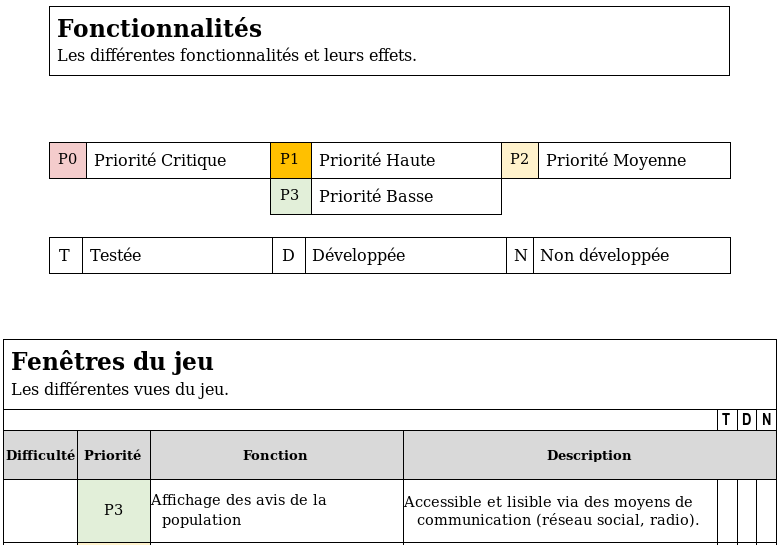
\includegraphics[width=1\linewidth]{figures/cdcf.png}}
      \end{figure}
      
      Une copie du cahier des charges est donné à la ou les personnes nommés 
      pour vérifier et donc tester que chaque fonctionnalité décrite existe 
      et marche exactement comme décrit.
      
      Si le la fonctionnalité est testée et validée, une croix est donc mise 
      dans la colonne \code{T}.
      
    \subsection{Notes}
      Toutes ces exigences ont été définies par les membre du projet et validées 
      par le chef du projet. Aucune exigence ne nous a été donné ou imposé par
      des membre extérieur à notre groupe.
           
      
    \section{Identification des facteurs de risques}

      \subsection{Load balancing: autoscaling}
        Si la sortie de données est plus élevée que de \texttt{1.25 Gbps} sur une instance donnée,
        une nouvelle instance est invoquée afin de répartir la charge imposée.
        
        La raison que cette valeur a été choisie, est qu'elle répond bien à notre cas :
        \begin{itemize}
          \item Instance avec peu de ressources et donc sensible (1GB) ;
          \item Instance avec peu de coeurs et donc de threads (2 threads) disponibles 
                pour absorber la charge sans accrocher ;
          \item Mais c'est une application légère qui lit qui ne fait rien d'autre que lire 
                un tableau en mémoire RAM.
          \item $ 3\mu s $ par requête, qui, chacune génère 2 octets compressés en GZip.
        \end{itemize}
        
        Nous n'avons donc que de simples variables avec un logiciel très puissant et optimisé
        qui ne fait rien de compliquer qui pousse les ressources. Mais, si cela arrive (ex. \emph{DDoS}),
        le serveur saura comment absorber si les sécurités anti-DDoS n'ont pas été assez réactives.
        
      \subsection{L'intégration logiciel}
        Le problème de l'intégration logiciel ne se pose pas, 
        le jeu n'aura besoin de rien d'autre que lui-même pour fonctionner 
        (un simple \code{.exe} contenant toutes les références statiques des dépendances). 

      \subsection{Le multiplateformes}        
        En ce qui concerne l'aspect multiplateformes, 
        le jeu sera disponible sous Windows, Linux et Mac.
        Les différents champs en entrée de texte sont limités à 40 caractères.
        
      \subsection{Facilité d'utilisation et cohérence}
        Le jeu est très simple d'utilisation. 
        Pour la cohérence graphique, nous avons une image d'arrière-plan, 
        et les personnages au second plan, puis le texte et menu au premier.
        
      \subsection{Gestion des erreurs internes}
        En cas d'erreur, le joueur est invité à nous envoyer l'erreur par courriel 
        en un seul clique 
        (sans afficher les détails de l'erreur à l'écran, autrement l'utilisateur sera perdu).
        
        Le joueur peut soit fermer la fenêtre ou nous envoyer l'erreur. 
        Il peut continuer à jouer dans les deux cas.

      \subsection{Le temps de réponse}
        \begin{itemize}
          \item Maximum $ 50ms $ quand le joueur instruit de passer au texte suivant ;
          \item Maximum $ 2s $ lorsque le joueur change de scène 
                (chargement d'une partie, d'une nouvelle partie, etc.)
        \end{itemize}
        
        Il y a un cas où nous tentons d'accéder à internet 
        (si l'utilisateur à accepter notre contrat de vie privée, en respect avec la \emph{RGDP}).
        Cet accès à internet pour récupérer des données se lance en arrière-plan en asynchrone,
        tous les éléments à l'écran concerné par ces données se mettent en position d'attente
        (ex. ont le texte "chargement..."). Mais l'utilisateur ne ressentira pas le moindre
        ralentissement ou accrochage grâce au fait que cela se fait en arrière-plan.
        
        Nous imposons un chargement de ces informations à être fait sous $ 500ms $ 
        dans le cas d'une personne avec une bonne connexion internet (3G+).

      \subsection{Cas critiques}
        Le jeu doit pouvoir rester jouable même si :
        \begin{itemize}
          \item l'utilisateur manque de mémoire RAM, 
                et joue donc avec 1 GB ou plus de données dans la SWAP.
          \item l'utilisateur est déconnecté d'Internet.
        \end{itemize}

      \subsection{Sécurité des données}
        \begin{itemize}
          \item Toutes les données allant sur le cloud sont avec l'accord préalable du joueur ;
          \item Toutes les données envoyées et stockées sont anonymes, 
                il n'est possible d'associer une personne à une donnée ;
          \item Les \emph{logs} d'accès sont stockés et sont à caractère personnel (et non pas nominatifs),
                les seules informations stockées sont : l'adresse IP et l'heure. 
                Ces informations sont gardées 1 an, en respect avec législature Française ;
          \item La base de données est automatiquement copiée via TLS
                vers un autre data center tous les soirs à minuit.
          \item Toutes les données stockées en local ne possèdent aucune donnée personnelle.
                Et ne peuvent être accédées depuis l'extérieur de la machine de l'utilisateur 
                ou via le cloud.
        \end{itemize}
        

  \section{Phase de tests à prévoir}
    \subsection{Les moyens de tests}
      Comme décrit précédemment, nous allons avoir deux types de tests :
		
		  \begin{multicols}{2}
			  \setlength{\columnseprule}{.5pt}
			
			  \centerline{\textbf{Les tests automatiques}}
			  \vspace*{\fill}
			
			  \begin{itemize}
			  	\item Faire un contrôle de la qualité sur chaque changement, via l'outil \code{codecov.io} ;
				  \item Assurer que le projet et la documentation compilent sur toutes les plateformes, 
				        via l'outil \code{travis-ci.org} (Linux et Mac) et \code{appveyor.com} ;
				  \item Assurer que toutes les fonctionnalités marchent, et sur toutes les plateformes,
				        via l'outil \code{travis-ci.org} (Linux et Mac) et \code{appveyor.com}.
  			\end{itemize}
			
  			\vspace*{\fill}
				
  			\columnbreak
				
  			\centerline{\textbf{Les tests manuels}}
  			\begin{description}
  				\item Faire un contrôle que tout les outils de tests automatiques (CI), 
		  		      sont complétés et réussis, 
	  			      en regardant directement aux badges de status du projet dans le \code{README} ;
			  	\item Assurer que toutes les fonctionnalités du cahier des sont testées :
				        il faut imprimer ou faire une copie du cahier et cocher la bonne case 
				        si la fonctionnalité est présente et marche totalement ;
  				\item Jouer au jeu et essayer de casser les choses puis faire un rendu global 
	  			      si le test est passé ou non.
		  	\end{description}
  			 \vspace*{\fill}
	  	\end{multicols}
	  	
	  	\subsection{Organisation de la phase des tests}
	  	  Il faudra, lors de chaque meeting, prévoir une période de tests, qui est la suivante :
	  	  \begin{description}
	  	    \item[Vérification des CI (tests automatiques),] 2 minutes ;
	  	    \item[Tests du cahier des charges,] 10 minutes ;
	  	    \item[Tests du logiciel (essayer de casser, chercher des problèmes),] 15 minutes.
	  	  \end{description} 
	  	  
	  	  \subsubsection{Les Dates}
  	  	  Les périodes de tests seront donc, les :
	    	  \begin{itemize}
	    	    \item 12 novembre 2018 ;
	  	      \item 19 novembre 2018 ;
	  	      \item 03 novembre 2018.
  	  	  \end{itemize}
  	  	  
  	 \subsection{Fiche modèle de tests}
  	   Vous retrouverez à la page suivante, notre fiche de compte rendu de tests.
  
  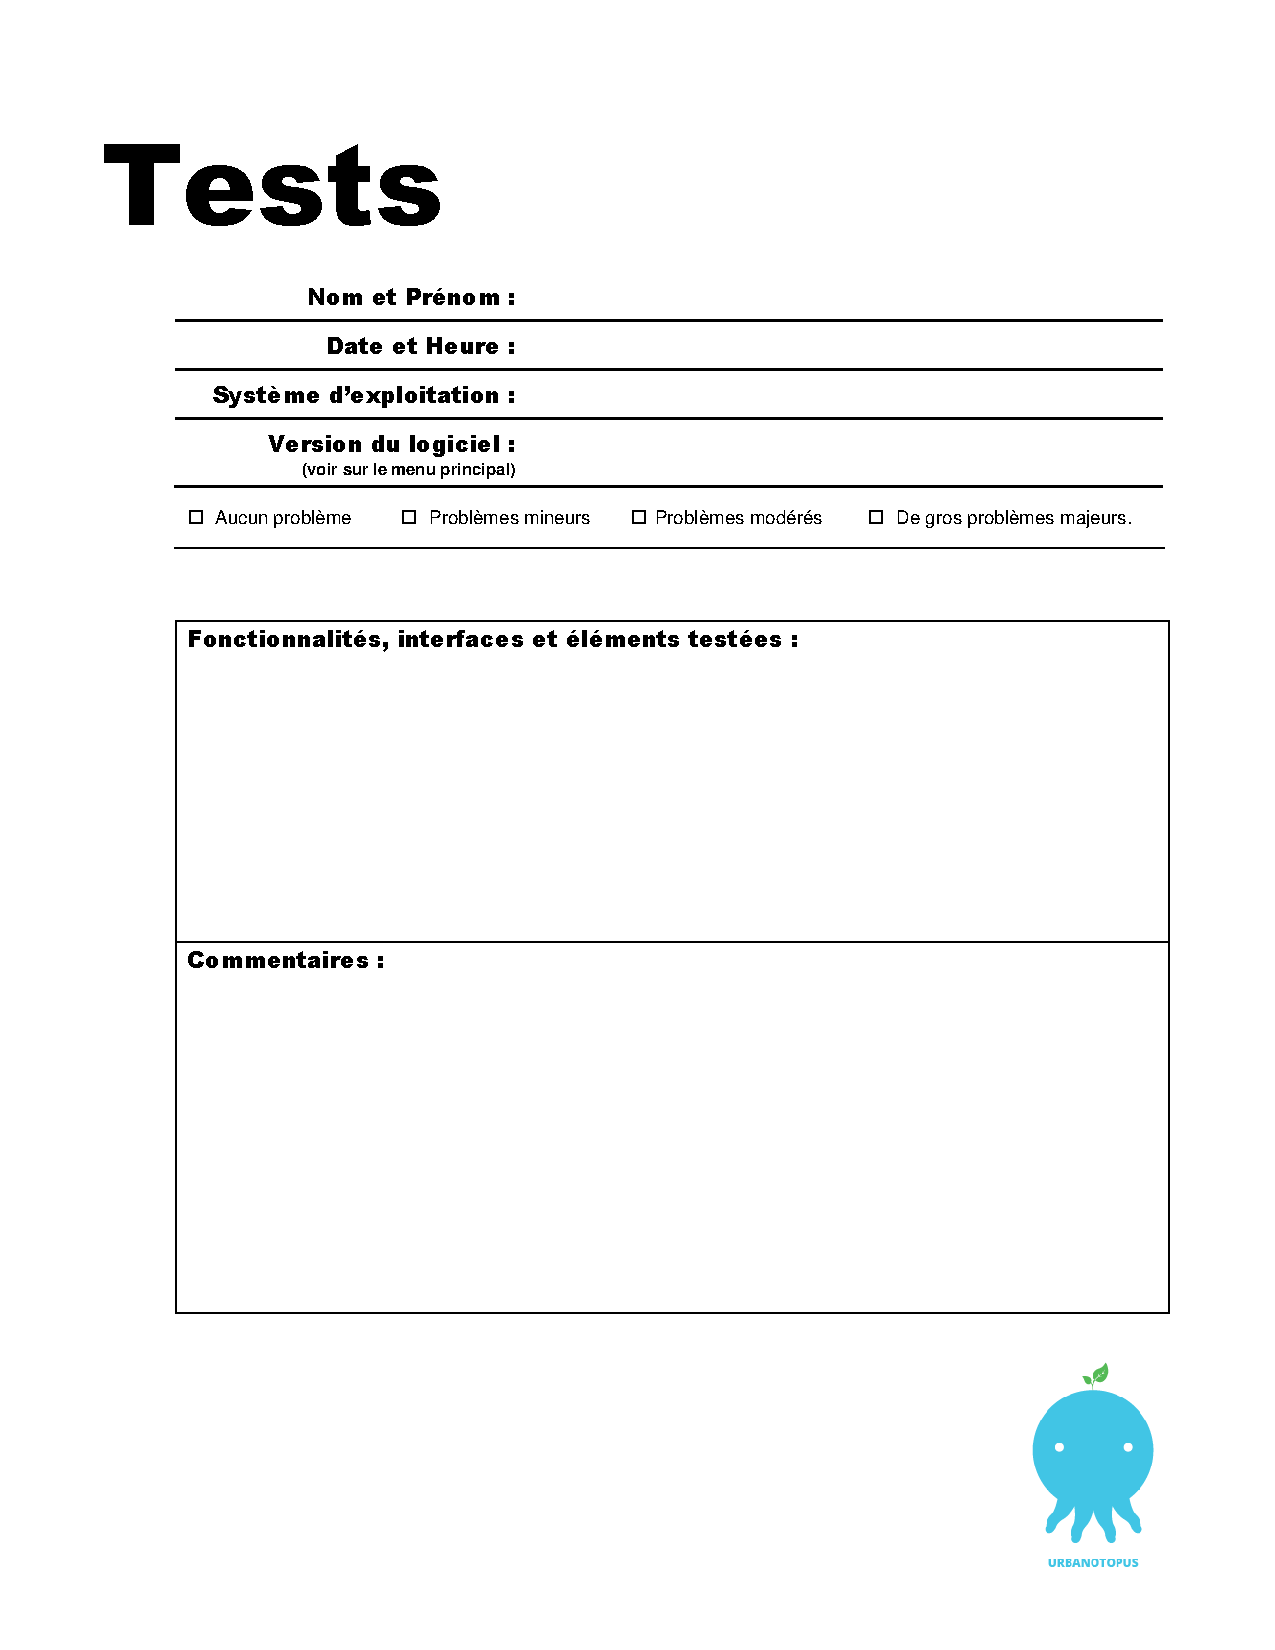
\includepdf[pages=-]{figures/revutests.pdf}
  
  
  \section{Conclusion}
    Nous avons entrepris ce projet avec les tests en priorité maximale avec un respect total 
    des dates limites. Et nous avons beaucoup misé sur une documentation aussi complète que possible,
    dans le but d'être un projet open-source ouvert aux contributions extérieures.
    Voici comment les temps a été utilisé au sein du projet :\\
    
    \begin{tabular}{ 
        | m{8.5cm} 
        | >{\centering\arraybackslash}m{1.5cm} 
        | >{\centering\arraybackslash}m{2cm} 
        | >{\centering\arraybackslash}m{0.6cm}
        | 
    }
      \hline
      Quoi ? & KOCAK & GROSJEAN & Loïc \\ \hline
      Recherches et planification des mécanismes de base du jeu & \multicolumn{3}{|c|}{(groupe) 3h} \\ \hline
      Recherches et planification sur le moteur du jeu & 6h & - & - \\ \hline
      Recherches et développement de solution d'intégration du CI dans le moteur & 7h & - & - \\ \hline
      Développement des mécanismes de base du jeu & 4.4h & 5h & 5h \\ \hline
      Développement du coeur du jeu & 5.3h  & - & - \\ \hline
      Écriture des scénarios & - & - & 5h \\ \hline
      Écriture, organisation et déploiement automatique de la documentation & 10.5h & - & - \\ \hline
      Total & 36.2h & 11h & 13h \\ \hline
    \end{tabular}
    
    
    \vspace*{\fill}

    \centering Notre documentation : \code{https://urbanotopus.readthedocs.io}
    
    ~
    
    \centering \qrcode[height=4cm]{https://urbanotopus.readthedocs.io/en/latest/index.html}
    
    ~\\
    
      
\end{document}
